\chapter{Adaptive Learning Strategies}\label{approach}

This chapter explains our approach for adaptive neural paraphrase generation. It describes the main learning strategies we use in detail including what purpose do they serve in our human-in-the-loop setting. We start with details of the model we use in our experiments, followed by the descriptions of datasets and evaluation metric we use. Then we explain learning strategies and discuss the experimental setups.

\section{Model Details}

In this work, we are using a lightweight variant of the model proposed in the work of \cite{Prakashetal} with bahdanau attention \cite{bahdanau}. The reason we are not using the exact same model is to fully explore all learning strategies since even with a lightweight version of the model, training takes a long time. In our model we keep the same stacked LSTM based multi-layer architecture with residual connections but we use 3 layers instead of 4. Figure 3 shows the basic unit in our model.

\begin{figure}[t]
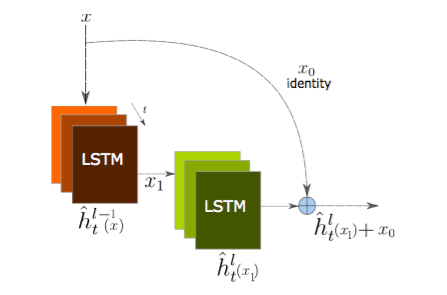
\includegraphics[width=\textwidth]{residualLSTM}
\centering
\caption{Stacked LSTM based model \cite{Prakashetal}}
\end{figure}


During experiments, the model has 512 units in each LSTM layer with dropout probability of 0.3 after each layer. We train our own word embeddings with the embedding size of 512. For all experiments learning rate is started with 0.001 and decayed exponentially with square root function.

In the cases when it improves performance we use beam search with beam size of 5.

\section{Datasets and Evaluation Metric}

We use four different datasets in our experiments varying in context and complexity. 

Microsoft Research Paraphrase Corpuus (MSR) \cite{msrp} is a small but very challenging dataset which contains 5800 pairs of paraphrases extracted from news sources. Since the paraphrase pairs are extracted from different news sources the dataset contains a lot of lexical and contextual variety. It also contains a lot of special words and concepts. Because of these reasons MSR corpus is a very hard dataset to create paraphrases from even by the state-of-the-art model with high computational resources. We separate the dataset into subsets of 2753, 997 and 150 for training, test and validation respectively.

Quora Question Pairs (QUORA) is a dataset consisting of question pairs which are labeled as paraphrases. It is originally a dataset for paraphrase recognition not paraphrase generation. We filter the positive class of dataset and collect 155,000 paraphrase pairs. There are one to many relationships in the dataset which means it contains multiple paraphrases for same source text. This property makes the dataset an ideal candidate for paraphrase generation. We separate the dataset into subsets of 119445, 22861 and 2000 for training, test and validation respectively.

Microsoft Common Objects in Context (MSCOCO) \cite{mscoco} is a large dataset consisting of human generated image captions with 351,163 pairs. It also has one to many relationships. MSCOCO is one of the most popular datasets used in paraphrase generation literature. We use all of the dataset for training.

PPDB Lexical (PPDB) \cite{ppdb} is a large dataset which contains 500,000 pairs of short paraphrases and it is also very popular in paraphrasing research. The paraphrases in this dataset are short therefore lack context information. We use all of the dataset for training.

\begin{table}
\small
 \begin{tabular}{||c c c c||} 
 \hline
 Label & Sentence & Dataset & \\ [0.5ex] 
 \hline
 source & the dvdcca then appealed to the state supreme court & MSR & \\
 \hline
 target & the dvd cca appealed that decision to the us supreme court & MSR & \\
  \hline
 source & why do rockets look white & QUORA & \\
 \hline
 target & why are rockets and boosters painted white & QUORA & \\
 \hline
 source & a blue and white bathroom with butterfly themed wall tiles & MSCOCO & \\
 \hline
 target & an angled view of a beautifully decorated bathroom & MSCOCO & \\
 \hline
 source & despicable & PPDB & \\
 \hline
 target & contemptible & PPDB & \\
 \hline
\end{tabular}
\caption{Example paraphrase pairs}
\end{table}


Table 3.1 shows example paraphrases from all the datasets we use. As it can be seen from the table, the datasets are varying in paraphrase complexity therefore it is easy to see why MSR dataset is harder to paraphrase from than the others. We use MSR and QUORA datasets as our target datasets, building and evaluating our models on them whereas we use MSCOCO and PPDB as source datasets to transfer from.

There are no evaluation metrics specifically designed for paraphrase generation. Therefore for evaluation we use the metric BLEU \cite{Papinenietal} which is a widely used metric for paraphrase generation. It is seen as a suitable option for paraphrase generation since it is shown that the score correlates well with human evaluation.

\section{Experimental Setups}

We simulate a human-in-the-loop data acquisition process by randomly dividing a dataset into train, test and validation, taking its subsets and feeding it to the model in each iteration. After each iteration we train the model with data we have according to learning strategy we experiment with and evaluate its performance with a separate test set (same test set for every iteration). The test sets are preferred to be relatively large in order to test how well the model generalize after each iteration. We train the model with same amount of epochs and start the training with same hyperparameter configurations through the iterations in order to compare the performance without bias. If it is necessary, parameter tuning is done on validation set beforehand and the best model is taken for experiment with learning strategies. Every learning strategy is experimented with the same model (same architecture, same hyperparameters etc.).

\section{Incremental Learning Strategies}

Considering our setting even though the training data is limited at the beginning, with time we are going to be able to use enough data to build a stable model even with supervised learning. In other words if we wait a certain amount of time, collecting data, we could train the model with supervised learning and use it for application purposes but by doing that we would not be using the training data available for a specific period of time which could be very long depending on the task and model. Moreover we would have to train the model on regular basis just to keep up with the training data. This is not desirable and practical even impossible depending on the circumstances. Therefore, incremental learning is a natural option in our case.

Main concern in our setting is making continual, data-driven learning possible since traditional supervised learning is not possible. The model should keep learning with incoming training data which is provided by the data stream, adapt itself to the changes in dataset without forgetting the knowledge it learned before. Since the model is getting training data in small chunks, one of the most important design decisions we have to make is how to process available training data through time. In case of neural models learning basically means to update model's weights by iterations according to the training data. Because of the very nature of gradient descent based learning the more we use certain data points in training more the model is going to adjust itself towards to those data points. This could lead to a bias towards the training data which is gathered at past, severely hurting the model's learning capability. It is important to notice that this can also happen within the same dataset if the dataset has high variance. This problem would not occur if we train the model with supervised learning since we would have the whole dataset available.

As explained in previous sections, concept drift is the other big challenge we have to consider when learning in continuous data streams. Optimally model should be able to pick up the statistical and conceptual changes in the incoming training data and update its weights accordingly. The model should be able to do this without forgetting previously learned knowledge meaning that it should still be able to perform reasonably well when it comes across with test data drawn from datasets which are similar to early training distributions otherwise it would be meaningless to use it in real world applications since the model has no adaptivity. 

It is reasonable to say that when the two problems described above are considered, adaptivity of a model is basically a tradeoff between how fast it learns the new knowledge and how fast it forgets the old one. Any learning strategy that is to be used in adaptive learning, should employ some measures in order to preserve the balance between learning and forgetting. As it is said before because of the very nature of how deep neural models learn, it is impossible to avoid either one of them but it is possible control the rate of how fast the model learns and forgets. We propose and experiment with two different incremental learning strategies which differ in how they process the incoming training data. We also regulate the model with different methods available in traditional supervised learning. We study the behaviour of these two incremental learning approaches and try to provide insight on adaptive learning in NLP, more specifically paraphrase generation. The training and regularization methods we use are fairly simple but haven't been studied before so with our findings we would like to create a foundation for more complex approaches for adaptive NLP models.

\subsection{Incremental Learning with Data Pooling (IL1)}

First learning strategy we propose trains continuously (weights are not re-initialized between iterations, model uses and updates the same weights) from a data pool which contains all the data collected in previous iterations. The model uses all data available to it regardless how old or new the data is. Figure 3.1 shows the basic work flow of the learning strategy. As it can be seen from the figure at the end of each iteration, the collected data is placed in a data pool and the model trains itself using the updated data pool. After the training process next iteration starts and cycle continues. Purpose of this learning strategy is mainly show that if the neural model can constantly improve itself through time with the incoming data. Main focus is not to forget previously attained knowledge while learning new training data reasonably well and make model to use all the resources available. Some of the advantages and disadvantages of this type of learning are:

\begin{figure}[t]
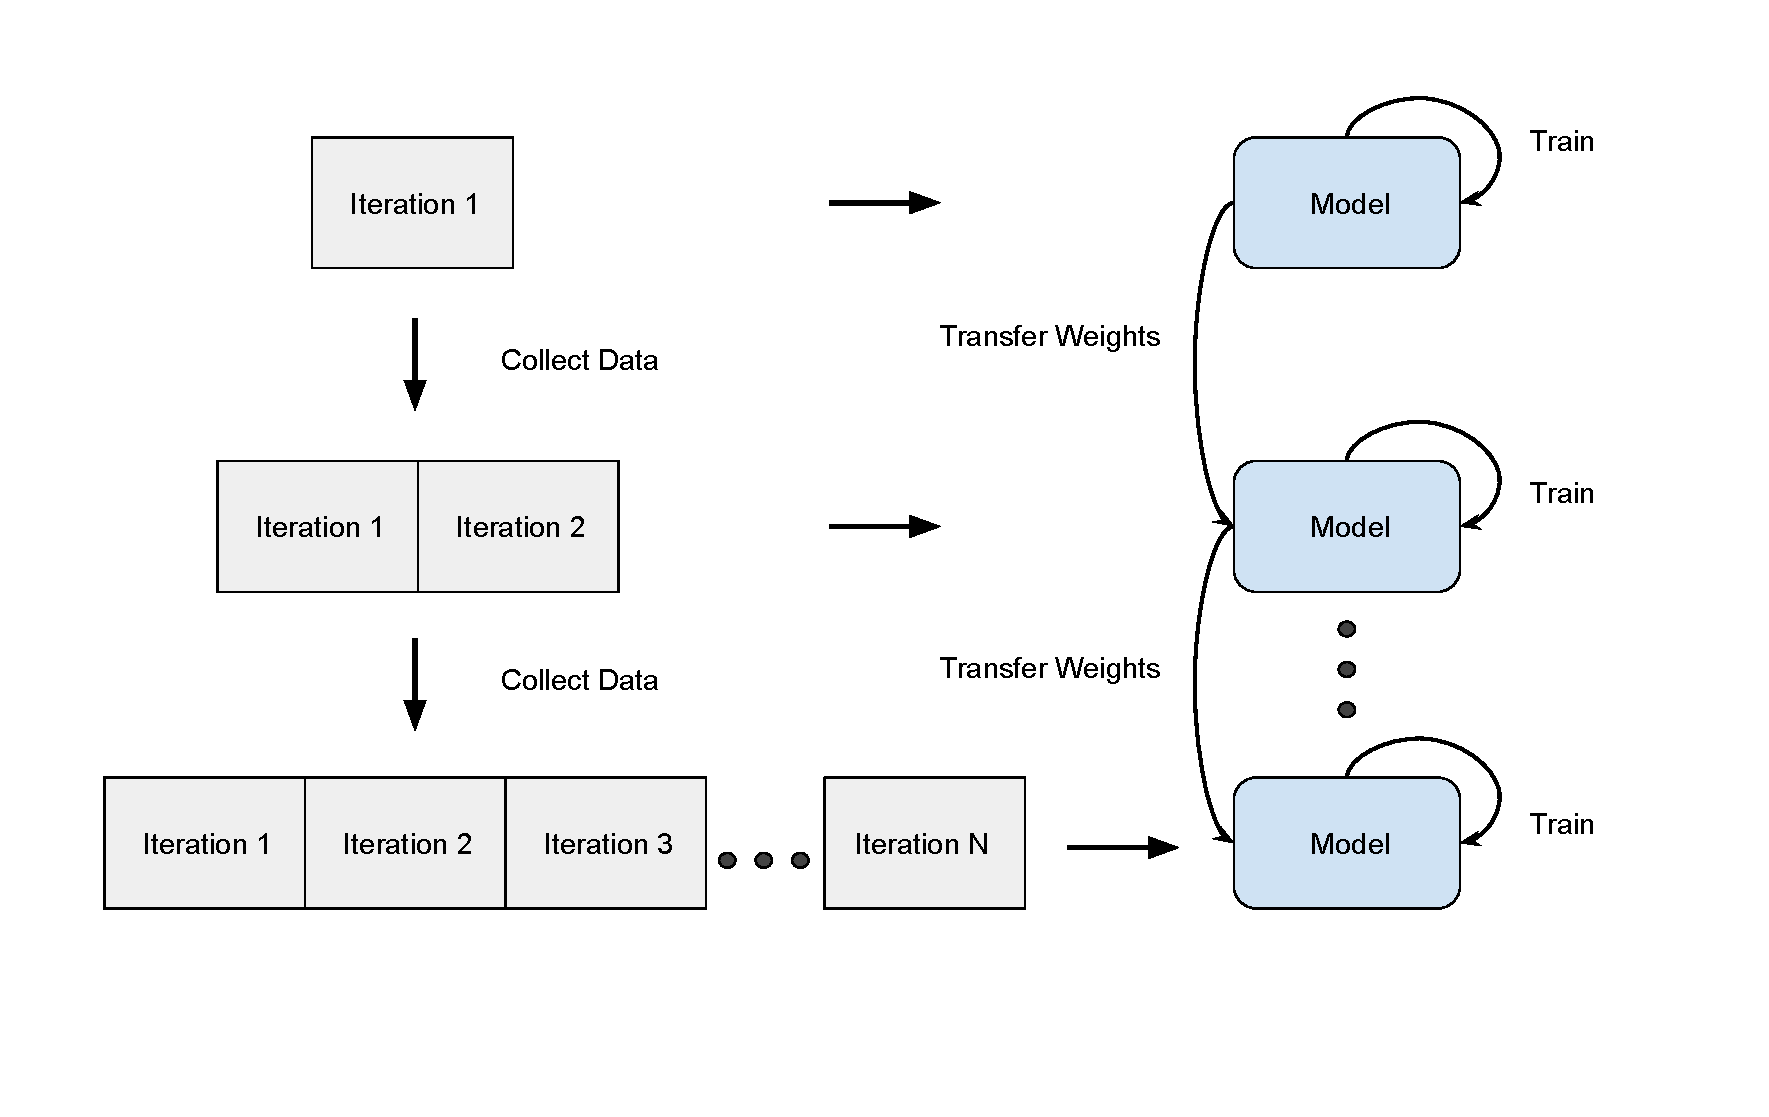
\includegraphics[width=\textwidth]{IL1}
\centering
\caption{Incremental learning with data pooling. The model uses data from all prevous iterations, hyperparameters re-initialized and weights are transferred through iterations.}
\end{figure}

\begin{itemize}

  \item Since the model trains on all data available at the end of each iteration, it is unlikely to forget learned knowledge from previous iterations.
  \item The model has the chance to learn more difficult data points better especially if they are encountered in early iterations. Basically instead of waiting to get enough data to learn with supervised learning, we can use that time to work on challenging data points we see.
  \item Since the size of data pool is increasing linearly, the time model takes to the end of each iteration and the required memory for data pool, increases linearly as well.
  \item The model sees data points from earlier iterations way more often which means it updates its weights according to those data points more often. This can cause overfitting to those particular data points which can diminish the performance of the model.

\end{itemize}

\subsection{Incremental Learning without Data Pooling (IL2)}

Second learning strategy we propose trains continuously (weights are not re-initialized between iterations, model uses and updates the same weights) only from the data of last iteration. There is no data pool that aggregates collected training data. Figure 3.2 shows the basic work flow of the learning strategy. As it can be seen from the figure, the model only updates itself with the most recent iteration. After the training process next iteration starts and cycle continues. Purpose of this learning strategy is to create an efficient model in terms of training time and memory. Main focus is the adaptivity of model to new data. Some of the advantages and disadvantages of this type of learning are:

\begin{figure}[t]
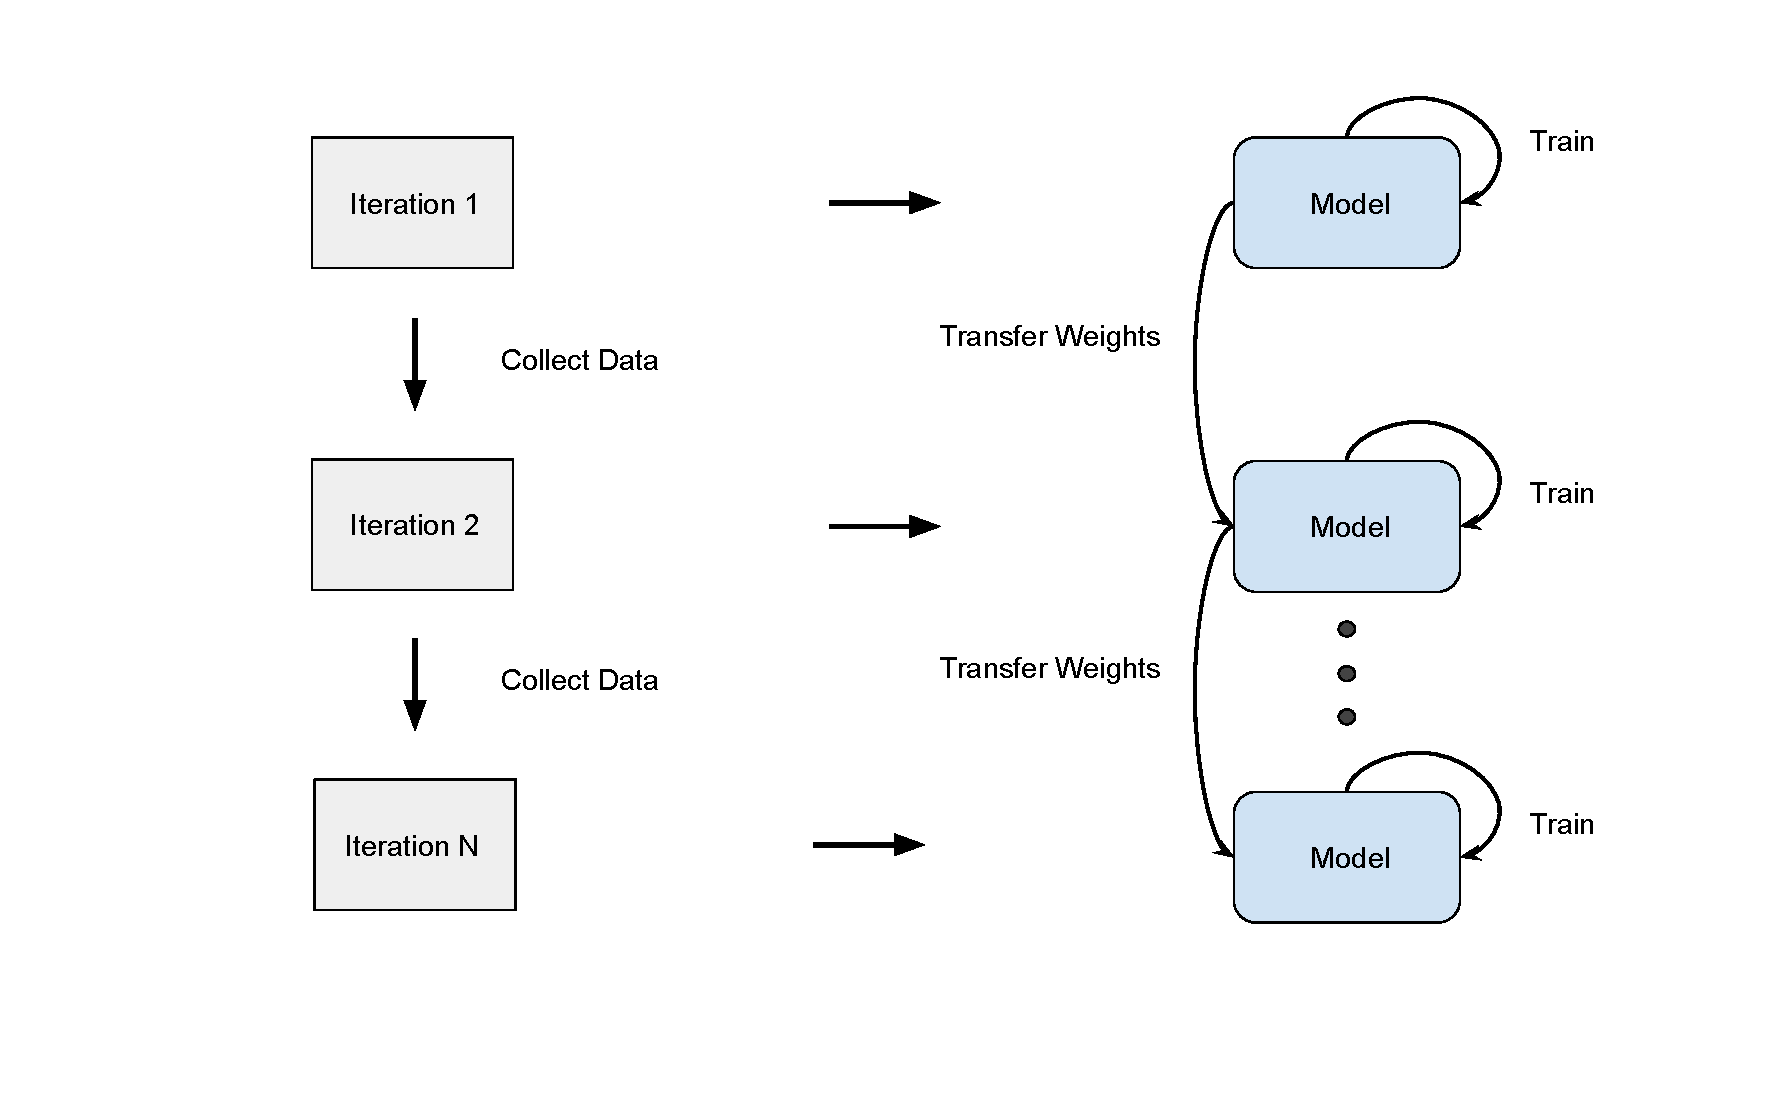
\includegraphics[width=\textwidth]{IL2}
\centering
\caption{Incremental learning without data pooling. The model only uses data from latest iteration, hyperparameters re-initialized and weights are transferred through iterations.}
\end{figure}


\begin{itemize}

\item Since the model trains on iterations separately it is prone to overwrite and forget old knowledge from previous iterations.
\item All training points are updated for same amount of iterations. If the number of epochs are not large enough the model can underfit and fail to generalize.
\item Since the size of data pool is constant, it is efficient in terms of time and memory.
\item The model sees all data points for equal amount of times therefore it does not have the problem of overfitting as incremental learning with data pooling.

\end{itemize}

\subsection{Incremental Learning with Network Expansion (IL-NE)}

Last learning strategy we propose trains continuously (weights are not re-initialized between iterations, model uses and updates the same weights) and expands the neural network after certain number of iterations. In this context network expansion means adding another LSTM layer to the network. Purpose of this learning strategy is to increase adaptive capabilities of the model. Main focus is to deal with possible concept drift which can occur during data acquisition. By adding randomly initialized new layers when more than certain amount of data is introduced to the model, we try to create specialized layers focusing on old and new information. We experiment with expansion in every third iteration and expansion only in the fifth iteration. We also experiment with freezing first active layer in every expansion step, studying if restricting the model through time helps with adaptivity. Figure 3.4 shows the basic workflow of this freeze and expand process.  

\subsection{Incremental Learning Baseline (IL3)}

We also train the model from ground zero (with the weights re-initialized) from data pool at the end of every iteration in order to create a comparable baseline. The baseline model which is trained after the last iteration is basically the model trained with supervised learning since it uses the whole training data available. We check if the incremental learning strategies achieve better or comparable performances than last baseline model.

\begin{figure}[t]
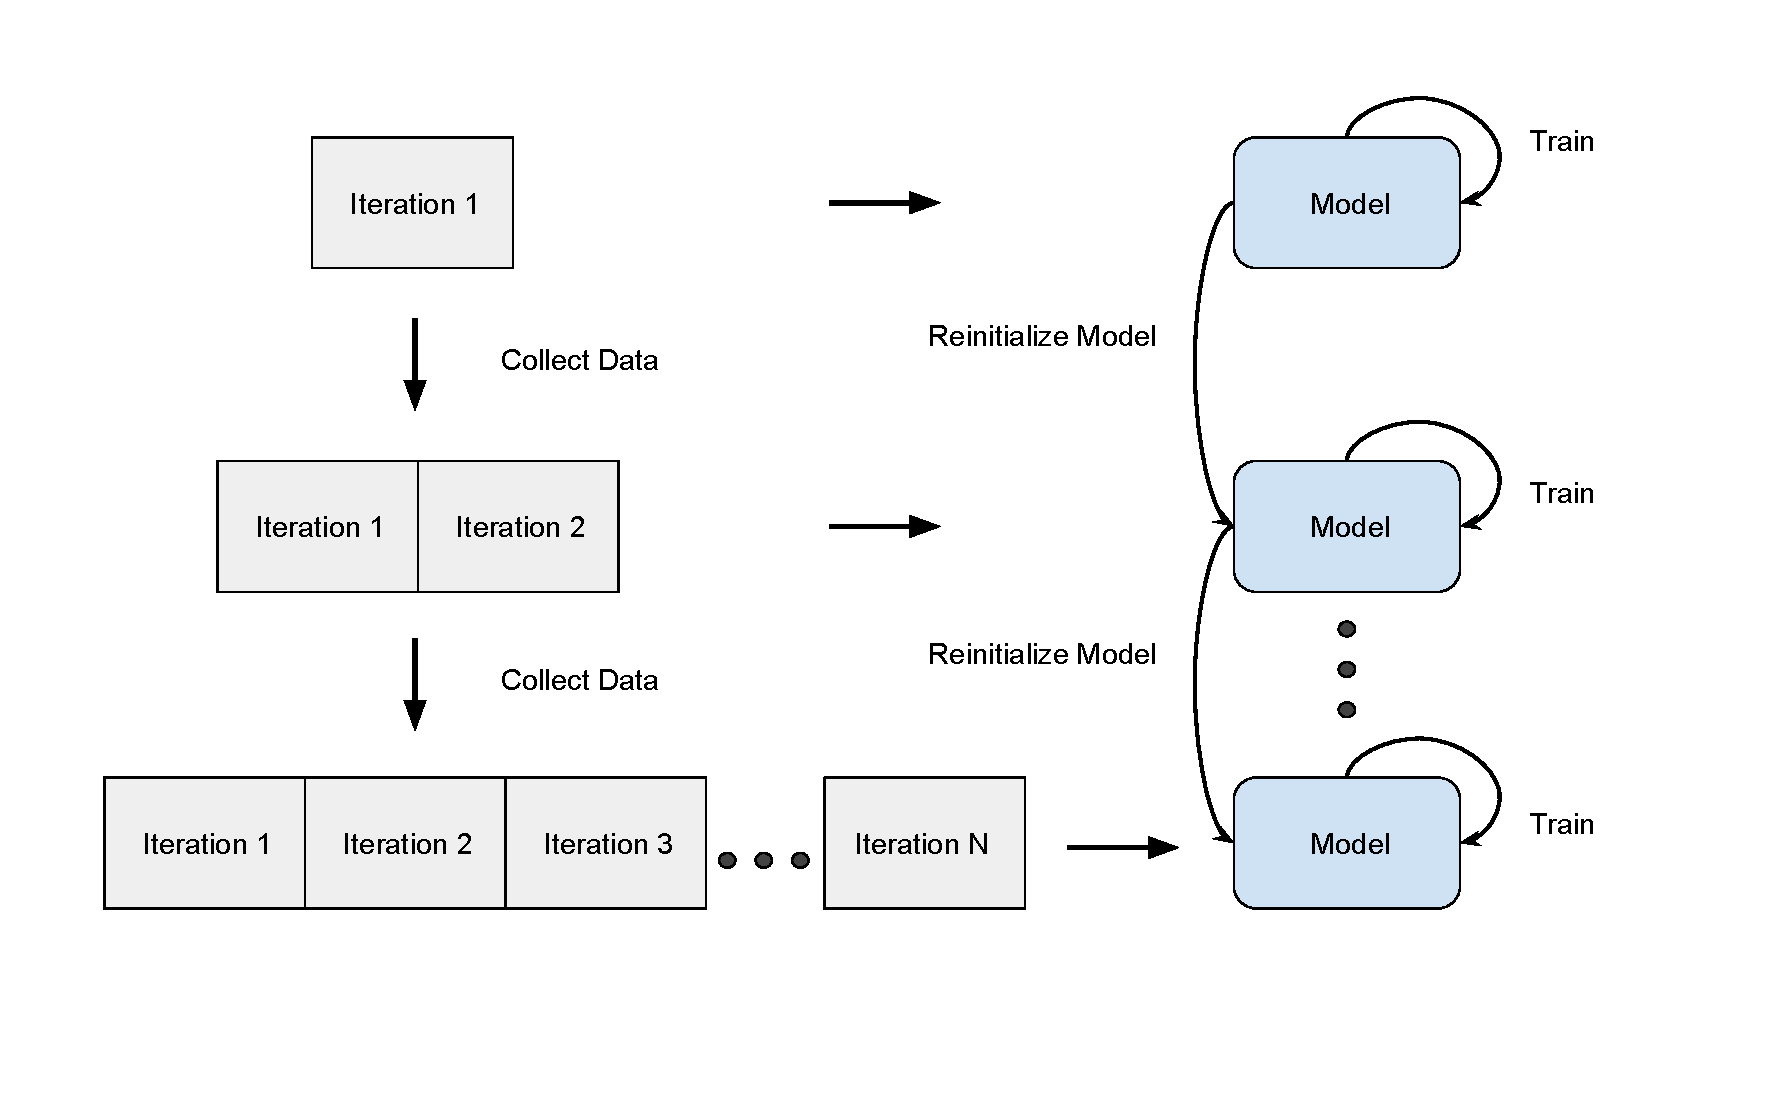
\includegraphics[width=\textwidth]{IL3}
\centering
\caption{Incremental learning baseline. The model is trained from scratch for each iteration, no knowledge transfer involved.}
\end{figure}

\subsection{Model Regularization in Incremental Learning}

We use simple and well known regularization techniques with incremental learning strategies in order to control the tradeoff between old and new information. Regularization techniques we use in our models are dropout, learning rate decay and layer freezing. Learning rate and its decay is used to control how large the weight updates are during the learning. We purpose non-shared the learning rate and decay rate for every iteration of training in order to make the model adaptive to most recent data. We make the assumption that a very small learning rate with high decay rate will make the model unresponsive to the latest iterations. We use exponential learning rate decay (square root decay) in our experiments which means the learning rate will decrease through an iteration. We use dropout to prevent overfitting especially in incremental learning with data pooling where the model is updated for certain data points way more than the rest of dataset. We also freeze certain number of the layers so that corresponding layers' weights are not updated during training. We make sure that some of the previously learned knowledge is not overwritten by the incoming dataset. 

\section{Transfer Learning Strategies}

During incremental learning we train the model at the end of each iteration with training data specified by the incremental learning strategy we use. Since we are training the model continuously without re-initializing the weights in each iteration we are basically doing transfer learning between iterations. In our initial experimental setups, the training data comes from the same dataset divided into subsets provided as iterations. We would like to expand this experiment setup by transferring knowledge from a different paraphrasing dataset and start the incremental learning process with a pre-trained model or in other words with a knowledge base. 

Transfer learning from other sources are extremely relevant to our continuous human-in-the-loop setting especially in the cases where we don't have resources to collect a large dataset. Since the training data is collected iteratively the model would have to work with even smaller dataset at the beginning. Transfer learning can help the model learn better, providing a better initialization in the worst case scenario and increase the performance in this case. More importantly by training a model in a different dataset and using the pre-trained model to learn a new dataset basically an artificial equivalent of concept drift no matter what transfer strategy is used. Basically, in this case we have model which is used for a different dataset (different statistics, distribution, context etc.) than the one it is trained with. Only difference between this scenario and the concept drift scenario we have in incremental learning is in this case we have access to all of the new dataset, instead of small chunks. Therefore finding good strategies for transfer learning can help with concept drift if the transfer strategies is combined with incremental learning. 

Before starting with the transfer learning from other paraphrase datasets, we run experiments for answering these questions:

\begin{itemize}

\item Is knowledge transfer possible for neural paraphrase generation?

In order to answer this question, we train a model with a large paraphrasing dataset as a source model. Then we transfer from this source model to target model with simplest way possible which is copying the weights of every component of source model and train the target model in supervised manner. We compare the performance with traditional supervised learning and see if there is any improvement.

\item If answer to the first question is yes, what components of the model is being transferred?

To see what aspects of the source model is transferred we run experiments with three different settings; transfer embedding layer only, transfer embedding and hidden layers, transfer all layers including output layers. We compare the performances and see what components lead to improvement. 

\item Does transfer success depend on the characteristics of participant datasets?

In order to speculate about what properties of the datasets relevant to knowledge transfer, we run experiments with three different source datasets and two target datasets. We study the transfer performance and establish some correlations between performance and properties like context, content, size of the datasets.

\end{itemize}

After establishing knowledge transfer is indeed possible, as it can been seen from Figure 3.6 we propose three different transfer strategies:

\begin{itemize}

\item INIT: Knowledge transfer is done by copying every component of source model to target model.  

\item Freeze n-layers: Same as INIT but first n layers of the model are freezed.

\item Surplus layer:  Same as INIT but a surplus layer is added before output layer and all the other layers are freezed.

\end{itemize}

Basically, proposed transfer strategies is designed for putting restrictions on the source model, directly effecting how much the model learns from training data. Whereas INIT puts no restrictions on the target model, surplus layer conservatively keeps the knowledge from source model and freeze n-layers approach is thought as a middle ground between them, making adjustments between knowledge learned from source dataset and target dataset . With transfer learning the model deals with a similar old vs. new knowledge tradeoff as incremental learning but with a different scale. In this case old knowledge part of the tradeoff is much larger and can have significant effects on the models performance. Moreover all of the transfer strategies proposed in this chapter are designed while specific use cases are considered. We hypothesize that INIT is more suitable when the dataset for target model is large and the model has to be complex whereas surplus layer is more suitable when the dataset for target model is small and the model has to specialize (general to specific for the same domain). 

We use the same regularization techniques as incremental learning strategies for transfer learning strategies even though their effect on the performance can be not the same. Since it is essential to efficiently use the knowledge learned from source dataset in target dataset, learning rate for the target model becomes very important. I large learning rate might overwrite the existing weights very quickly which means losing the information gained before. Therefore in our experiments we used larger learning rate for source dataset and smaller learning rate for target dataset. We keep the same exponential learning decay we used in incremental learning.

\section{Active Learning Strategies}

Active learning is perfectly suitable for human-in-the-loop setting since it aims to enable learning with lees amount of. Not only it can reduce the cost of data acquisition, it can also enhance the overall process since it enables the model to learn faster which would mean earlier and more meaningful involvement with the users. As it is explained before the core idea behind active learning is determining the most difficult data points to paraphrase and make the users annotate those data points. We aim to integrate active learning into our incremental learning with data pooling strategy and study its effects on model's performance. We hypothesize that since incremental learning with data pooling updates its weights towards to some data points in the dataset more than others, if those points are made sure to be most difficult data points to paraphrase, this can help the model to train better and faster.

It is hard to define a difficult or informative data point in case of paraphrase generation just because of the fact that it is a generation task not classification or regression. Contrary to other NLP tasks like paraphrase recognition or named entity recognition, in paraphrase generation we only have the source texts to work with which limits the information we have on the dataset. For example in the case of paraphrase recognition, the dataset contains both of the paraphrase pairs and the annotator is only have to decide if they have the same meaning or not but nevertheless information from both of the sentences can be used for sampling. In our case we base our sampling strategies only on the source texts which consists of two heuristics and model's opinion. We combine four different sampling strategies and incremental learning with data pooling. Sampling techniques we use for our experiments are:

\begin{itemize}

\item Random Sampling (RS): Sentences which are going to be paraphrased by the user are selected randomly. This is the default method for all of the other experiments in this thesis and used as a baseline.

\item N-gram Coverage (NC): Proposed in \cite{rubio} for interactive machine translation, this sampling technique focuses on selecting the rarest data points in terms of their n-grams. In other words, this technique aims to calculate how much new information a data point can provide. The hypothesis is rarest sentences have to be seen more for model to learn an accurate probability estimation. 

Before the training number of each n-gram present in the training data, is calculated and stored. Since human-in-the-loop approach is simulated, n-gram counts of the whole dataset can be calculated beforehand but in a real world application where new training data is constantly streamed, they should be updated after each iteration. We label an n-gram rare when it appears less than A times in training data. Using this label we compute the score for a given source sentence f as:

\begin{equation}
C(f) = \frac{\sum_{n=1}^N \lvert{\nu^{<A}_{n}(f)} \lvert} {\sum_{n=1}^N \lvert{\nu_{n}(f)} \lvert} 
\end{equation}


where ${\nu_{n}(f)}$ is the set of n-grams with size n in f, ${\nu^{<A}_{n}}$ is the set of n-grams of size n in f that are rare and N is the maximum n-gram order. In experiments with incremental learning with data pooling, N = 4 is chosen as the maximum n-gram order and a value of 10 is chosen for the threshold A. In order to asses how well n-gram coverage represents the informativeness of data we also experiment with reverse n-gram sampling where the data points are chosen based on how frequent they are in the dataset in terms of n-grams. The score for reverse n-gram sampling is calculated as:

\begin{equation}
C(f) = \frac{\sum_{n=1}^N \lvert{\nu^{>=A}_{n}(f)} \lvert} {\sum_{n=1}^N \lvert{\nu_{n}(f)} \lvert} 
\end{equation}

where the terms are the same as n-gram sampling equation.

\item Least Confidence (LC): A very intuitive sampling technique, it chooses data points in which the model has least confidence in. In the context of deep neural models this means to select the data points that are assigned with lowest probability according to the equation \cite{shen}:

\begin{equation}
1 - \max_{y_{1}.....y_{n}}  \mathbb{P}  \left[ {y_{1}.....y_{n}}  | \{ x_{ij} \}  \right]   
\end{equation}

For LSTM based sequence-to-sequence model used in this work, the score for a data point is calculated by using the probability of greedily decoded sequence.

\end{itemize}

Since MSR dataset contains a very small size, we only try active learning strategies on QUORA dataset.


